%----------------------------------------------------%
%       ANÁLISIS DE LAS TÉCNOLOGÍAS PROPUESTAS       %
%----------------------------------------------------%

\pagestyle{fancy}

\chapter{Análisis de las tecnologías propuestas}
\label{analisis_tecnologias}

\section{Apache Cassandra}

Apache Cassandra es una base de datos distribuida que permite operar sobre grandes volúmenes de datos del tipo clave/valor. Se caracteriza por ofrecer una  disponibilidad total y mayor escalabilidad lineal en comparación a otras bases de datos NoSQL, utilizando, para ello, una serie de nodos homogéneos que se comunican mediante un protocolo P2P de replicación asíncrona, lo cual permite realizar operaciones de baja latencia para todos los clientes sin necesidad de un servidor maestro.\\

Fue concebida en el 2008 por los ingenieros de Facebook basándose en sistemas de almacenamientos distribuidos como Dynamo (Amazon) \cite{decandia2007dynamo} y BigTable (Google) \cite{chang2008bigtable} con el propósito de mejorar la funcionalidad de búsqueda en la bandeja de entrada. En 2012, investigadores de la Universidad de Toronto que estudian los sistemas NoSQL concluyeron que "En términos de escalabilidad, hay un claro ganador a través de nuestros experimentos. Cassandra logra el mejor rendimiento para el número máximo de nodos en todos los experimentos" \cite{rabl2012solving}. Hoy en día, el mayor impulsor del proyecto es DataStax \footnote{\url{http://www.datastax.com/}}, empresa que operando bajo la licencia de Apache \footnote{\url{http://www.apache.org/}} desarrolla tanto ésta base de datos como una infinidad de herramientas que facilitan el uso de la misma.\\

Actualmente Apache Cassandra es utilizada por infinidad de aplicaciones en negocios modernos, siendo la base de datos elegida por un tercio de las compañías que conforman la Fortune 100 \footnote{\url{http://fortune.com/2015/04/14/datastax-hp-sales-partnership/}}. Claro ejemplo de ello son empresas mundialmente conocidas como Apple, Facebook o NetFlix, los cuales utilizan Apache Cassandra como parte de su entramado tecnológico desde hace ya unos años. Cabe destacar que el uso del mismo no se limita al mundo empresarial. Muestra de ello es la acogida que ha tenido en el ámbito de la investigación, formando parte en experimentos punteros a nivel mundial como algunos de los realizados en el CERN \cite{sicoe2012persistent}.\\

\subsection{Funcionamiento}

Las bases de datos NoSQL, en su mayoría, han sido concebidas para lidiar con un conjunto especifico de problemas. Debido a ello, para entender el funcionamiento de Apache Cassandra se ha decidido resaltar las peculiaridades que le distinguen de los demás sistemas de almacenamiento no relacionales.

\subsubsection{Base de datos distribuida de alta disponibilidad}

El Teorema de Brewer \cite{gilbert2002brewer}, también conocido como Teorema CAP , enuncia que un sistema de cómputo distribuido no puede  garantizar simultáneamente las tres propiedades que se presentan a continuación, solo pudiendo cumplir dos de ellas al mismo tiempo, y acabar cumpliendo la restante tarde o temprano:

\begin{itemize}
	\item \textbf{Consistencia}(Consistency): Todos los nodos ven la misma información al mismo tiempo.
	\item \textbf{Disponibilidad}(Availability): La garantía de que cada petición a un nodo reciba una confirmación de si ha sido o no resuelta satisfactoriamente.
	\item \textbf{Tolerancia al Particionado}(Partition Tolerance): El sistema sigue funcionando a pesar de que haya sido partido por un fallo de red.
\end{itemize}

Para una base de datos distribuida que promete la disponibilidad completa, el Teorema de Brewer implica la incapacidad de garantizar la consistencia total de los datos que almacena y la necesidad de esperar un tiempo indeterminado para que las réplicas de un registro modificado se actualicen correctamente.\\

Para lidiar con dicha restricción, Cassandra ofrece la posibilidad de afinar el nivel de consistencia \footnote{\url{https://docs.datastax.com/en/cassandra/2.1/cassandra/dml/dml_config_consistency_c.html}} en cada consulta sacrificando para ello parte de la disponibilidad. Las consultas de mayor disponibilidad responden con el dato ofrecido por la primera réplica en contestar sin siquiera cotejar la existencia de una versión actualizada del mismo, mientras que las consultas de mayor consistencia podrán fallar por la caída de un nodo que alberga una de las réplicas debido a no poder satisfacer el nivel de consistencia requerido. Por tanto, queda en manos del diseñador el trabajo de encontrar el equilibrio entre ambas características, siendo la naturaleza de los datos a tratar un factor determinante para ello.

\subsubsection{Optimizado para escrituras}

Una de las características a destacar de Cassandra es el elevado ratio de escrituras por segundo que es capaz de realizar, superando notoriamente a otras bases de datos NoSQL en este apartado \cite{rabl2012solving}.

Al ejecutar una consulta que desemboca en una escritura, los registros son almacenados en dos estructuras denominadas CommitLog y Memtable. El primero, es un fichero donde se adjuntan los registros recibidos, mientras que el segundo, es una cache en memoria que apila dichos registros hasta llegar a su capacidad máxima. Sólo cuando ambas estructuras finalizan de guardar los datos, Cassandra considera que la consulta ha sido ejecutado satisfactoriamente pudiendo pasar a procesar otras operaciones.\\

Cuando la Memtable se llena empieza un proceso de vaciado en el cual, primero, se dilucida el nodo destinatario de cada registro. Después, dichos registros son escritos de forma secuencial en estructuras inmutables denominadas SSTable, ficheros que representan físicamente el contenido de una tabla en Cassandra. Si esta operación es interrumpida, se utiliza la información almacenada en el CommitLog para recuperar las escrituras perdidas. Finalmente, cuando todos los registros han sido transferidos su correspondiente SSTable el CommitLog es purgado.\\

\begin{figure}[h]
	\centering
	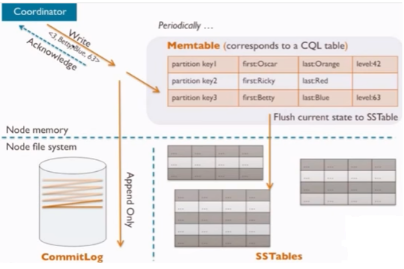
\includegraphics[width=0.65\textwidth]{Ilustraciones/cassandra_data_storage.png}
	\caption{Almacenamiento de datos en Cassandra}
	\label{fig:almacenamiento_cassandra}
\end{figure}

Debido a la naturaleza inmutable de las SSTable, cada vez que la Memtable se vacía un nuevo fichero es generado para representar una misma tabla. Ello puede conllevar problemas de eficiencia a la hora de consultar la información de dicha tabla, ya que será totalmente necesario leer todos los ficheros correspondientes. Para sobreponerse a este inconveniente, Cassandra posee un mecanismo llamado compactación.

\subsubsection{Replicación asíncrona sin maestro}

//Gossip Protocol (paper?)

Protocolo de comunicación peer-to-peer que intercambia el estado del propio nodo y de aquellos cuyo estado conoce de forma periódica.

El proceso es ejecutado cada segundo e intercambia información con otros tres nodos del cluster. De esa forma, todos los nodos aprenden sobre el resto de manera rapida.

Cada mensaje Gossip tiene una versión asociada a él, gracias al cual el nodo que recibe dicho mensaje puede comparar con la información que tiene y sobreescribir su conocimiento en caso de ser necesario.

//Failure Detector (paper?)

Necesidad de diferenciar un nodo caído con otro en estado transitorio para redireccionar las peticiones solo a los nodos activos.

El detector de fallos es un método que permite determinar localmente si otro nodo del sistema esta caido o en funcionamiento mediante el uso de los estados gossip y el historial.

Cassandra utiliza accrual detection mechanism para calcular un umbral por nodo que tenga en cuenta el rendimiento de red, carga de trabajo, u otras condiciones.

Es posible configurar dicho umbral modificando el valor de la variable phi_convict_threshold para ajustar la sensibilidad del detector de fallos.

// merkle tree (paper?)

Consiste en comparar todas las réplicas de cada dato que existe o debería existir y actualizarlos a la versión más reciente mediante el uso de Merkle Trees.

Un Merkle tree es un árbol de hash donde los nodos padres más altos en el árbol son los hashes de sus respectivos hijos. La ventaja principal de árbol de Merkle es que cada rama del árbol se puede comprobar de forma independiente , sin la necesidad de descargar todo el conjunto de datos.

La implementación de Anti-Entropia de Cassandra genera un Merkle tree por cada column family a la hora de la compactación y se almacenan solo hasta enviarlos a los nodos vecinos. 

Implica enviar un exceso de datos por la red pero ahorra en operaciones I/O del disco local, lo cual es preferible para conjuntos de datos muy grandes.

\subsubsection{Sin punto único de fallo}

//replicacion factor + diapositivas

///

Analizando las características propias de Cassandra y en concreto su estructura, la Keyspace es un espacio de nombres para un conjunto de ColumFamily. Por lo general, se utiliza uno por aplicación y es considerado como el equivalente a una base de datos del modelo relacional. El ColumFamily, a su vez, es capaz de almacenar diferentes columnas, siendo el homólogo de una tabla del modelo relacional. Para finalizar, una columna está compuesta por clave y valor, además de un campo del tipo timestamp gracias al cual se actualizan las réplicas obsoletas.\\

\begin{figure}[h]
	\centering
	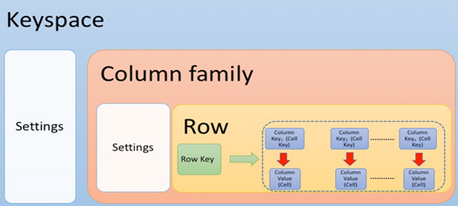
\includegraphics[width=0.5\textwidth]{Ilustraciones/cassandra_infraestructure.png}
	\caption{Estructura de Cassandra}
	\label{fig:cassandra_infraestructure}
\end{figure}

A la hora de definir un keyspace dos atributos estrechamente relacionados han de ser especificados: Replication Factor y Replica Placement Strategy(). El primero, consiste en un número que indica cuantas copias de un mismo registro se han de almacenar en la infraestructura. Cada nodo posee una réplica para un cierto rango de datos y si uno de ellos falla, otro que posea dicha réplica puede responder a la petición sin tener que interrumpir el servicio. El segundo, define cómo se han de repartir los registros replicados por el anillo, ofreciendo distintas opciones dependiendo si los nodos del clúster se encuentran alojados en un único datacenter o repartidos entre varios.\\

El atributo Replica Placement Strategy cobra especial interés al operar sobre un clúster cuyos nodos están distribuidos en punto geográficos lejanos, ya que permite almacenar cada réplica en diferentes puntos del globo. De esa manera, se consigue minimizar la latencia de las peticiones recibidas desde diferentes puntos del plantea y además, proteger la base de datos de una posible caída a nivel de datacenter debido a diversos catástrofes.\\ 

Si un componente de Cassandra tiene especial importancia en su funcionamiento es el ColumFamily. En una base de datos relacional como MySQL, las tablas son diseñadas con el objetivo de minimizar la redundancia de los datos almacenados en ella, siguiendo para lograr dicho objetivo un proceso de normalización[]. En cambio, al operar con Cassandra, ocurre exactamente lo contrario. Las tablas se construyen buscando una respuesta rápida a las consultas sin importar que ello implique tener que almacenar datos redundante en la base de datos.\\

patition key etc



\begin{figure}[h]
	\centering
	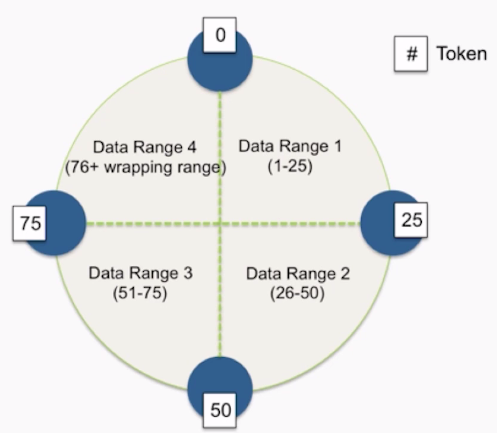
\includegraphics[width=0.5\textwidth]{Ilustraciones/cassandra_token.png}
	\caption{Particionamiento en Cassandra}
	\label{fig:cassandra_token}
\end{figure}

consecuencia: restriccion en las consultas que se pueden realizar

\subsection{Cassandra Query Lenguage (CQL)}

permite conectarse al cualquier nodo del cluter (homogeneidad)

Apache Cassandra posee su propio lenguaje de consultas, el denominado Cassandra Query Lenguage (CQL). Su sintaxis guarda una gran similitud con la de SQL, lo cual facilita, de forma notoria, el salto que supone pasar de trabajar con bases de datos relacionales a distribuidos.\\

Aún siendo sintácticamente  tan parecido a SQL, presenta ciertas restricciones debido a que es un lenguaje de consultas de una base de datos distribuida. Por ejemplo, no ofrece la posibilidad de realizar operaciones como JOIN y es totalmente necesario especificar todas los atributos que componen la clave primaria a la hora de realizar cualquier consulta de filtrado o de actualización en la tabla. La única operación que no cumple esta restricción es un select que contenga la clausula where, ya que, al definir la clave primaria Cassandra indexa de forma automática todos sus componente, posibilitando más tarde  hacer uso de ellos en este caso concreto.

Otra de las peculiaridades que presenta CQL es el hecho de ofrecer dos modos distintos de realizar un update. El primero de todos es el mencionado en el párrafo anterior. El segundo posibilita actualizar una columna realizando un insert repitiendo el valor de las claves primarias de una columna ya existente en la base de datos. Esta segunda forma es cómoda a la par de peligrosa porque Cassandra no notifica si una clave primaria ya existe en la base de datos o no, pudiendo un insert desencadenar en un update no deseado.  

\section{Apache Spark}

Apache Spark[9] es un proyecto open source de computación en clúster. Desde el principio fue diseñado para poder ejecutar algoritmos iterativos en memoria sin la necesidad de almacenar en disco los resultados intermedios generados durante el proceso. Esta peculiaridad permite que los procesamientos llevados a cabo con Spark puedan llegar a ser, en algunos casos concretos, 100 veces más rápidos que los de MapReduce[10].\\

A mediados de 2014, coincidiendo con el lanzamiento de la primera versión, alcanzó la cifra de 465 colaboradores, convirtiéndolo en el proyecto más activo entre los relacionados con el Big Data dentro de la Apache Software Fundation.\\

Apache Spark está compuesto por múltiples y variados componentes que pueden ser utilizados de forma conjunta.\\

\begin{figure}[h]
	\centering
	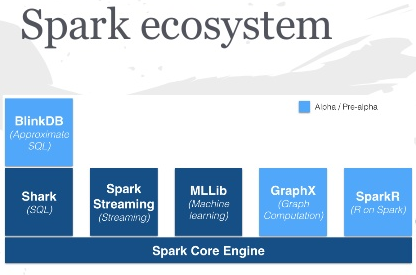
\includegraphics[width=0.5\textwidth]{Ilustraciones/spark_ecosystem.png}
	\caption{Ecosistema Spark}
	\label{fig:ipanel}
\end{figure}

La base del proyecto es el denominado Spark Core. Proporciona envío distribuido de tareas, planificación y funciones básicas de entrada salida. La abstracción fundamental de programación se llama Resilient Distributed Datasets (RDD)[11], una colección lógica de datos particionados a través de las máquinas que se expone mediante una API integrada en lenguajes como Java, Python y Scala.\\

\subsection{Funcionamiento}

Para el funcionamiento de Spark, es condición sine qua non que los nodos de la infraestructura tengan acceso a la totalidad de los datos que se desea tratar. Ello implica que para procesar un fichero de 50GB, cada nodo tendría que poseer una copia del mismo almacenado en su disco. Esta praxis es inviable, ya que más allá de los problemas de consistencia que generaría, para nada es eficiente ocupar la memoria de todos los nodos con información redundante y procesar el fichero entero cuando en realidad se va a hacer uso de una pequeña porción de dichos datos en cada ejecución.\\

Las bases de datos distribuidas como Cassandra solventan los problemas anteriormente mencionados. Se encargan de distribuir los datos entre diferentes nodos del clúster, ofrecen la posibilidad de acceder a ellos desde cualquier punto y mantienen la consistencia de los mismos a cambio de sufrir una pequeña latencia en el caso de requerir información almacenada en otro nodo de la infraestructura.\\ 

Al ejecutar una aplicación que opera con Spark, un componente denominado driver es lanzado. Debido a la necesidad de obtener recursos (CPU y memoria) para llevar a cabo la computación que se le ha encomendado, se comunica con un nodo del clúster que, mediante especificación previa, adopta el rol de maestro. Éste pregunta a todos los nodos que conforman la infraestructura sobre la cantidad de recursos disponibles que poseen y así asignarles los executors correspondiente. Las máquinas que alojen al menos un executor pasan a denominarse worker y a partir de este momento, cada executor podrá comunicarse directamente con el Driver para poder recibir las tareas que éste le envíe.\\

Un executor es una unidad de trabajo que se encarga de computar las tareas que le encomienda el driver. El número de executors que puede albergar cada worker está directamente relacionado con el número de procesadores que este posee. De la misma forma, es posible repartir la memoria RAM que dispone el nodo worker entre varios executors. Spark permite modificar ambos parámetros programáticamente permitiendo así poder amoldarse a las particularidades de cada ejecución.\\

Para transferir el código del programa, residente en la máquina del driver, éste adopta  el rol de servidor e intenta enviar dicho código a los workers. Si el fichero JAR que contiene el código ha sido recibido correctamente por sus destinatarios, estos responden mediante un ACK y en caso contrario, se vuelve a intentar el envío un número determinado de veces. Una vez llegado al máximo de reintentos, el worker que no haya enviado el ACK es considerado como caído, quedando los executors que albergaba fuera del posterior reparto de tareas.\\

\begin{figure}[h]
	\centering
	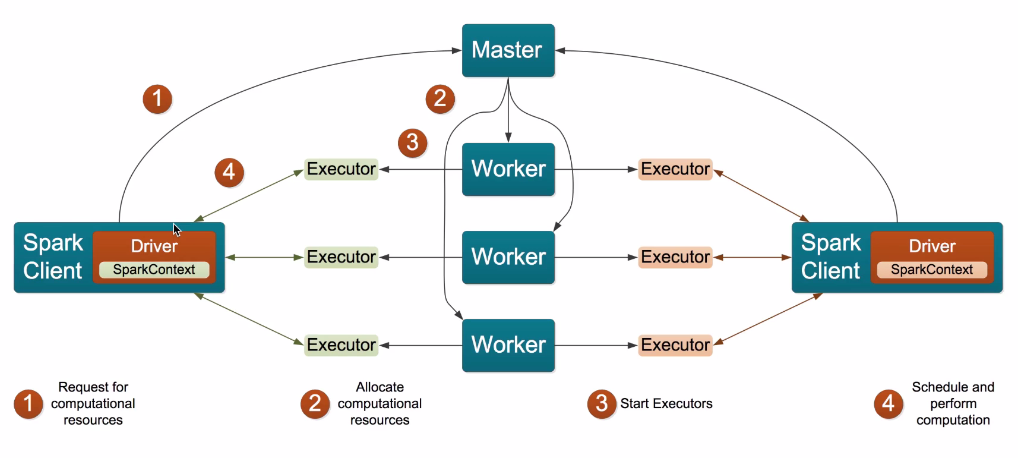
\includegraphics[width=1\textwidth]{Ilustraciones/spark_architecture.png}
	\caption{Arquitectura Spark}
	\label{fig:spark_architecture}
\end{figure}

A la hora de realizar operaciones en Spark, el objeto estrella es el denominado Resilient Distributed Datasets (RDD)[11]. Se trata de una abstracción que mediante diferentes APIs disponibles para Java, Scala y Python permite manipular datos distribuidos por los diferentes nodos del clúster como si estuvieran almacenados de forma local. Este objeto es inmutable, lo cual implica que una vez creado no se le pueden añadir nuevos elementos o eliminar los existentes, solo aplicar transformaciones y acciones sobre el.\\

Las operaciones que se pueden realizar sobre las RDD se agrupan, tal y como se ha adelantado antes, por transformaciones y acciones. Las primeras transforman un RDD en otro según el criterio indicado y las segundas realizan modificaciones sobre los datos almacenados en dichas RDD. Cabe destacar que las transformaciones en Spark son operaciones "lazy", lo cual implica que en realidad cada nodo memoriza la secuencia de transformaciones que ha de realizar y los procesa cuando una acción es ejecutada.\\

Una vez terminada la primera fase en la que los executor son creados y enlazados con el driver, éste último empieza a analizar la estructura del código y genera un grafo DAG (Directed Acyclic Graph) con las operaciones que se realizan sobre la RDD. Partiendo de ese grafo genera un job por cada operación de tipo acción que encuentra y dentro de cada job separa la ejecución en diferentes stages según las dependencias que existan entre operaciones. Por último, cada stage es dividido por defecto en unidades de 64MB y a cada unidad resultante se denomina task, el cual es enviado a un executor para ser procesado. El tamaño de cada task puede ser modificado programáticamente, pudiendo de esa forma manipular el número de task que un executor deba ejecutar.\\

\begin{figure}[h]
	\centering
	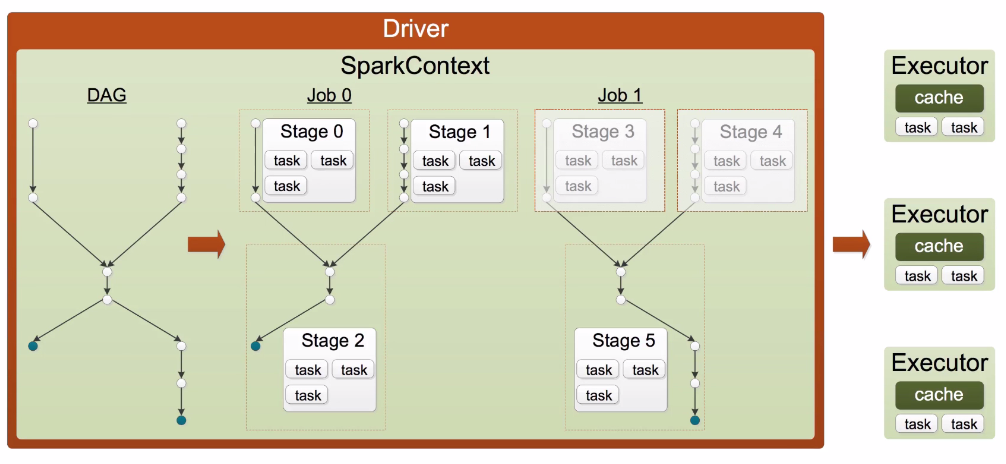
\includegraphics[width=1\textwidth]{Ilustraciones/spark_task_creation.png}
	\caption{Arquitectura Spark}
	\label{fig:spark_task_creation}
\end{figure}

El driver, una vez habiendo recibido los resultados de todas los task que ha repartido, enviará un mensaje a los executors indicando que el procesamiento ha sido finalizado y calculará el resultado final ofreciendo la posibilidad de, por ejemplo, almacenarlo en una base de datos distribuida como Cassandra.\\






